% !TEX encoding = UTF-8 Unicode
% !TEX root = rapport.tex

\part{Les conséquences d'évolutions divergentes}
Du constat de la dichotomie dans l'intégration de la technologie par la société et par l'éducation, émerge un questionnement : quelles sont les conséquences de ce décalage pour les individus ?

Pour tenter de répondre à cette question, nous allons examiner trois aspects de la société où les \gls{ticLabel} sont intégrées. Nous allons tout d'abord montrer pourquoi nous pensons que les formations dispensées à l'école sont en inadéquation avec les besoins des entreprises et pourquoi cela nuit-il aux individus. Nous allons ensuite nous pencher sur les retombées imprévues de l’utilisation des technologies de la communication dues à leur non intégration dans l'éducation. Enfin, nous chercherons des pistes pouvant expliquer en partie les décrochages et les échecs scolaires.



\chapter{Des formations en inadéquation avec les besoins des entreprises}
La faible intégration des \gls{ticLabel} dans l'éducation pose un certain nombre de problèmes quant à la pertinence des formations.

% les attentes de l'industrie
En effet, les attentes de l'industrie quant aux compétences d'un
individu se portent sur ses capacités à {\bf raisonner} et à {\bf être
  créatif}. Les recruteurs recherchent des candidats bilingues formés aux
\gls{ticLabel} et possédant de l'expérience en entreprise
\cite{DRH_criteres}. Au contraire, les facultés de calcul ou la
capacité à engranger des connaissances sont de moins en moins
appréciées. Savoir trouver ou retrouver rapidement les informations
utiles devient un besoin essentiel dans un monde où une grande part de
la connaissance est accessible a tout moment à travers le web.

% le contenu des formations
De nos jours les machines remplacent les départs en retraite dans les industries ; les ordinateurs calculent bien plus efficacement que les humains ; la fiabilité des technologies dépasse de loin celle des humains. Les postes nécessitant des compétences que possèdent aujourd'hui les machines sont déjà occupés et peu à peu fermés au profit des sus-mentionnées machines. Or, les formations dispensées ne sont pas fondamentalement différentes de celles du début du  \siecle{20} \cite{robinson2010paradigms} dans des contextes de révolution industrielle et du siècle des lumières. Les \gls{ticLabel} y sont peu intégrées et la réflexion et la créativité sont défavorisées au profit du calcul, de l'apprentissage formel\ldots L'éducation ne prépare-t-elle donc plus les étudiants à leur vie future \cite{formation_recrutement} ? Est-il possible d'être épanoui dans sa vie professionnelle sans cadrer avec les attentes de ses pairs et/ou de ses supérieurs ?

% arguments
Afin d'appuyer nos présomptions sur l'inadéquation des formations avec les besoins des entreprises, nous allons présenter un faisceau d'indices.

\section{Chômage des jeunes}
\begin{figure}[p]
\centering
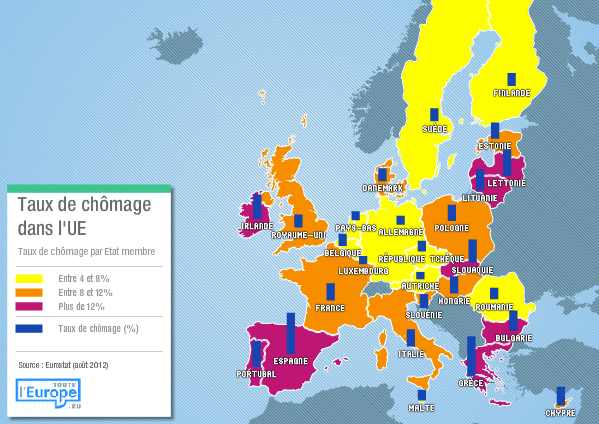
\includegraphics[width=0.98\linewidth]{../resources/illustrations/chom}
\caption{Taux de chômage dans l'UE en août 2012 \cite{chom}}
\label{chom}
\end{figure}
\begin{figure}[p]
\centering
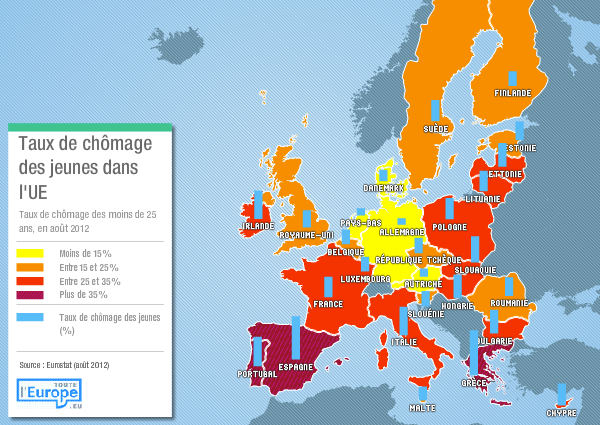
\includegraphics[width=0.98\linewidth]{../resources/illustrations/chom_jeunes}
\caption{Taux de chômage des jeunes dans l'UE en août 2012 \cite{chom_jeunes}}
\label{chom_jeunes}
\end{figure}
Commençons tout d'abord par examiner les données du chômage des jeunes comparées aux données globales du chômage (voir figures \ref{chom} et \ref{chom_jeunes}). Comme nous pouvons le constater, le chômage des jeunes est en moyenne deux fois plus important que le taux général du chômage en Europe. Cette disparité a de nombreuses explications dont certaines économiques. Nous pensons néanmoins que les causes dues à une formation inadaptée ne sont pas négligeables. 

En effet, les postes nécessitant une formation \og{}classique\fg{} sont déjà occupés. Les machines remplacent peu à peu les emplois industriels. Les recruteurs attendent donc des jeunes qu'ils aient d'autres compétences : celles que les machines ou les seniors n'ont pas.

Notons tout de même que le chômage est bien plus répandu chez les jeunes ayant une formation très courte que chez ceux possédant un diplôme du supérieur. La formation des plus jeunes à l'école de la république ne devrait-elle donc pas rendre adaptables les individus ?

D'autre part, l'air du temps pousse les jeunes à devenir entrepreneurs de par le manque d'emplois salariés. Or les moyens à leur disposition ne permettent pas à la plupart d'entre eux de monter une entreprise. Quant est-il de la place de l'esprit d'initiative au sein de notre société ?


\section{Difficulté des entreprises à recruter}
\begin{figure}[p]
\centering
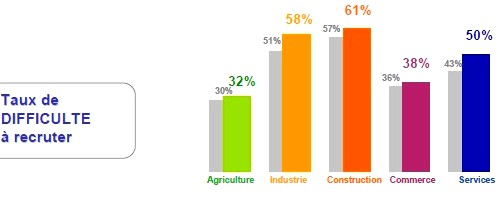
\includegraphics[trim=7cm 0cm 0cm 0cm, clip=true, scale=1]{../resources/illustrations/diff_recrut}
\caption{Difficultés à recruter par secteur en 2012 en Midi-Pyrénées \cite{recrutement_midi_pyr}}
\label{diff_recrut}
\end{figure}
\begin{figure}[p]
\centering
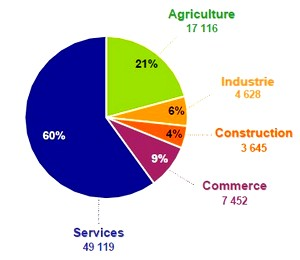
\includegraphics[scale=0.8]{../resources/illustrations/embauches}
\caption{Intentions d'embauche par secteur en 2012 en Midi-Pyrénées \cite{recrutement_midi_pyr}}
\label{embauche}
\end{figure}
Des rapports de pôle-emploi indiquent clairement que malgré le taux de chômage élevé, les entreprises ont des difficultés à recruter. En effet, il n'y a pas assez de candidats et ceux-ci ne sont pas assez compétents ou pas assez diplômés. 

Comme nous pouvons le constater sur les figures \ref{diff_recrut} et \ref{embauche}, les secteurs de l'agriculture, de l'industrie et de la construction manquent de vocations (ce qui peut s'expliquer par la rigueur du travail dans ces professions). D'autre part, les secteurs des services et du commerce ont également beaucoup de difficultés à recruter et cela peut s'expliquer par l'inadéquation de la formation des candidats avec les besoins des entreprises.

Nous pourrions nous demander si le rôle de l'école est bien de former des candidats aux besoins des entreprises. L'école n'est-elle pas plutôt censée élever les esprits et les âmes ? Toujours est-il que des individus jugés incapables de travailler correctement par leurs pairs et supérieurs ne peuvent pas être complètement heureux ! Le bonheur des individus au sein de la société n'est-il pas un objectif que l'éducation devrait viser ?


\chapter{Les retombées imprévues de l'utilisation des technologies de la communication}
Une mauvaise utilisation des \gls{ticLabel} et plus particulièrement des réseaux sociaux conduits bien souvent à des situations dramatiques. La plupart de ces situations pourraient être évitées par le biais de préparations et de formations des jeunes à l'impact réel des réseaux virtuels.

\section{Des embauches influencées par internet}
De plus en plus de recruteurs (surtout aux USA) tapent le nom des candidats dans un moteur de recherche internet avant de décider de leur embauche \cite{recrutement_internet, recrut_social_network, social_recrut}. Ce genre de recherche permet de trouver les profils des candidats sur les réseaux sociaux (généraux ou spécialisés pour l'embauche) mais également leur site internet ou de nombreuses informations sur leur vie.

\begin{figure}[H]
\center
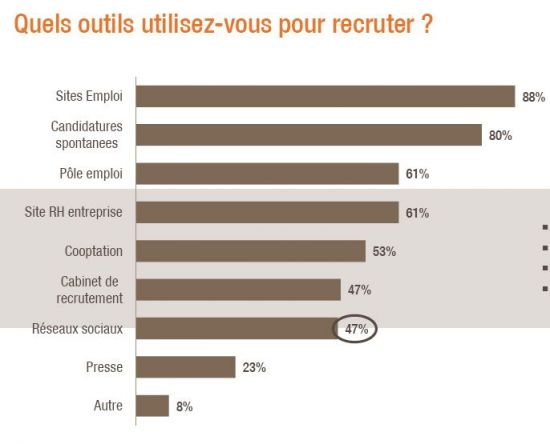
\includegraphics[width=0.8\textwidth]{../resources/illustrations/recrutement-enquete}
%% @todo need caption
\end{figure}
\begin{figure}[H]
\center
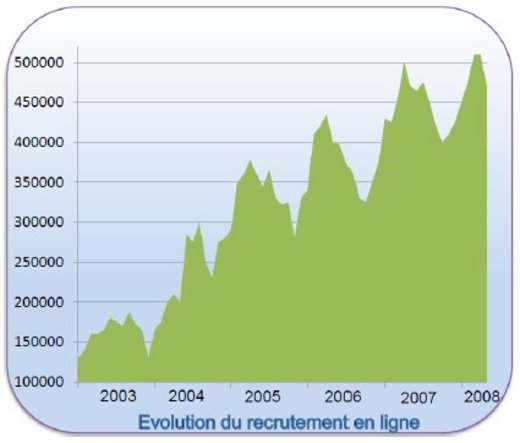
\includegraphics[width=0.6\textwidth]{../resources/illustrations/online_recrut}
\end{figure}

Or, si un candidat averti contrôle la diffusion des informations à son sujet sur internet, un non-averti peut diffuser des informations compromettantes pour une embauche. En effet, la publication d'un site web ou l'élaboration d'un profil sur des réseaux sociaux dédiés à l'embauche sont des points positifs ; tandis que des profils publics sur des réseaux sociaux généralistes peuvent contenir des photos, vidéos ou commentaires compromettants pour le candidat (comme des photos d'une soirées débridée ou un commentaire du candidat faisant du shopping pendant un après-midi ou il devrait être au travail par exemple).

Dans certains cas, des adolescents postent des photos et des vidéos
d'eux qui les rattrapent des années plus tard lorsqu'ils deviennent
adultes et rentre sur le marché de l'emploi.

%Une formation adaptée à l'utilisation des \gls{ticLabel} pourrait mener à une prise de conscience des dangers et à une responsabilisation des jeunes par rapport à ces technologies.

\section{Chantages, menaces et insultes sur les réseaux sociaux}
Les chantages, menaces et insultes sur les réseaux sociaux sont un des problèmes les plus importants liés à l'utilisation des \gls{ticLabel} sans formation. En effet la plupart de ces situations impliquent de jeunes adolescents qui n'ont pas conscience de la portée de leurs actes sur internet. Certains d'entre eux se déshabillent devant leur webcam, d'autres se confient à des inconnus. De ces imprudences résultent parfois des situations dramatiques comme par exemple le suicide de certains adolescents victimes de chantages ou de menaces \cite{chantage_facebook, harcel_facebook}.

\begin{figure}[h]
\hspace{-2cm}

\includegraphics[scale=1]{../resources/illustrations/Amanda_Todd}
\caption{Amanda Todd, adolescente Canadienne}
\end{figure}

Certains autres individus harcelés dans leur vie réelle voit le harcèlement se prolonger dans leur vie virtuelle. Certains autres postent des insultes sur divers réseaux sociaux sans se rendre compte de la portée de leurs actes.

%Encore une fois, tous ces problèmes pourraient être aisément évités en expliquant aux enfants la portée de leurs actes sur internet.



\chapter{Décrochages et échecs scolaires}
Les points que nous avons abordés précédemment mettent en évidence la nécessité d'enseigner mieux les tenants et les aboutissants des \gls{ticLabel}. Ceci doit être fait en ajoutant de nouveaux enseignements aux programmes scolaires.

Cependant, d'autres problèmes liés au manque d'intégration des \gls{ticLabel} dans l'éducation émergent et ceux-ci ne sont pas réglables par l'ajout de nouveaux enseignements aux programmes scolaires. Ainsi, nous allons essayer de percer à jour les causes du mal-être des élèves et des étudiants et ses manifestations : les décrochages et échecs scolaires.

\section{La formation des étudiants en inadéquation avec leurs attentes}
Comme nous l'avons déjà souligné, les paradigmes d'enseignement actuels n'ont guère évolués depuis le \siecle{19} \cite{robinson2010paradigms}. En effet, les professeurs enseignent et les élèves écoutent. Ce paradigme d'enseignement n'est plus adapté à la vie actuelle.

\begin{figure}[h]
\centering
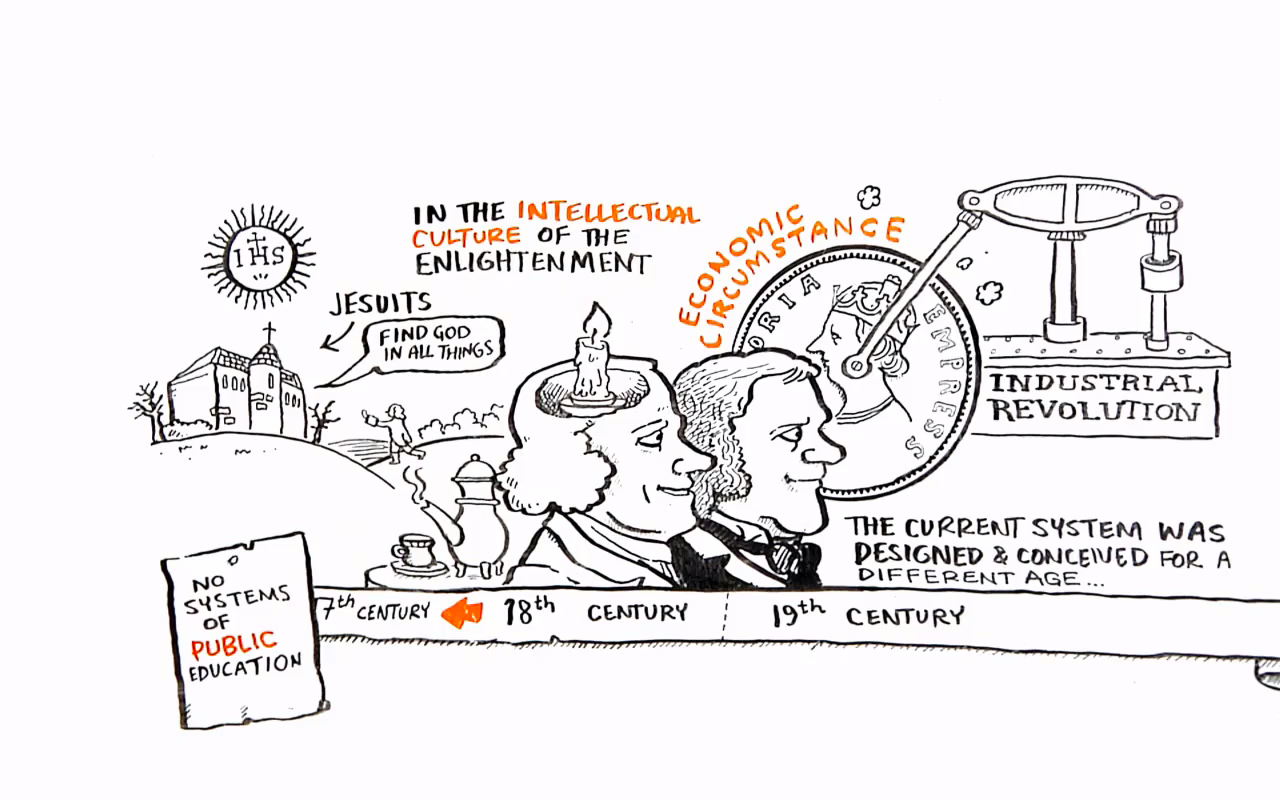
\includegraphics[trim=2cm 1.5cm 0cm 1.5cm, clip=true,
  width=\linewidth]{../resources/illustrations/public_education}
%% @todo need caption
\end{figure}

Les enfants des dernières générations ont grandi avec les nouvelles technologies aussi se sont-ils adaptés aux commodités qu'elles apportent. Ils ne voient plus l'utilité d'apprendre par cœur énormément d'informations quand ils peuvent juste y accéder en allant sur internet.

De plus, dans de nombreux cas, les formations ne sont pas suffisamment spécialisées : rabâcher les mêmes connaissances de base chaque année n'aide pas ceux qui ne les ont pas acquises à mieux les comprendre et démotive les autres.

Le regroupement des élèves par classe d'âge n'est pas pertinent. En effet, chaque élève a des besoins uniques et différents dans chacune des disciplines. Ne faudrait-il pas revoir l'intégralité des modes de fonctionnement~?

Enfin, les lacunes grandissantes des professeurs en ce qui concerne les nouvelles technologies ne facilite pas l'intégration de celles-ci par des initiatives locales.

Tous ces points problématiques mènent peu à peu au désintéressement des élèves et à la marginalisation de ceux qui ne peuvent s'intégrer sous ces conditions. Ainsi surviennent les échecs scolaires. Notre hypothèse est que l'intégration des nouvelles technologies dans l'éducation ainsi qu'une ré-évaluation des paradigmes d'enseignement pourraient régler ces problèmes.

\section{Hyperactivité et troubles de l'attention}
De nos jours sont diagnostiqués de plus en plus de troubles de l'attention avec hyperactivité. Ainsi, les prescriptions médicamenteuses visant à corriger ce trouble augmentent elles aussi. Comme le montre la figure \ref{adhd_map}, cela prend la forme d'une épidémie \cite{robinson2010paradigms}.
\begin{figure}[h]
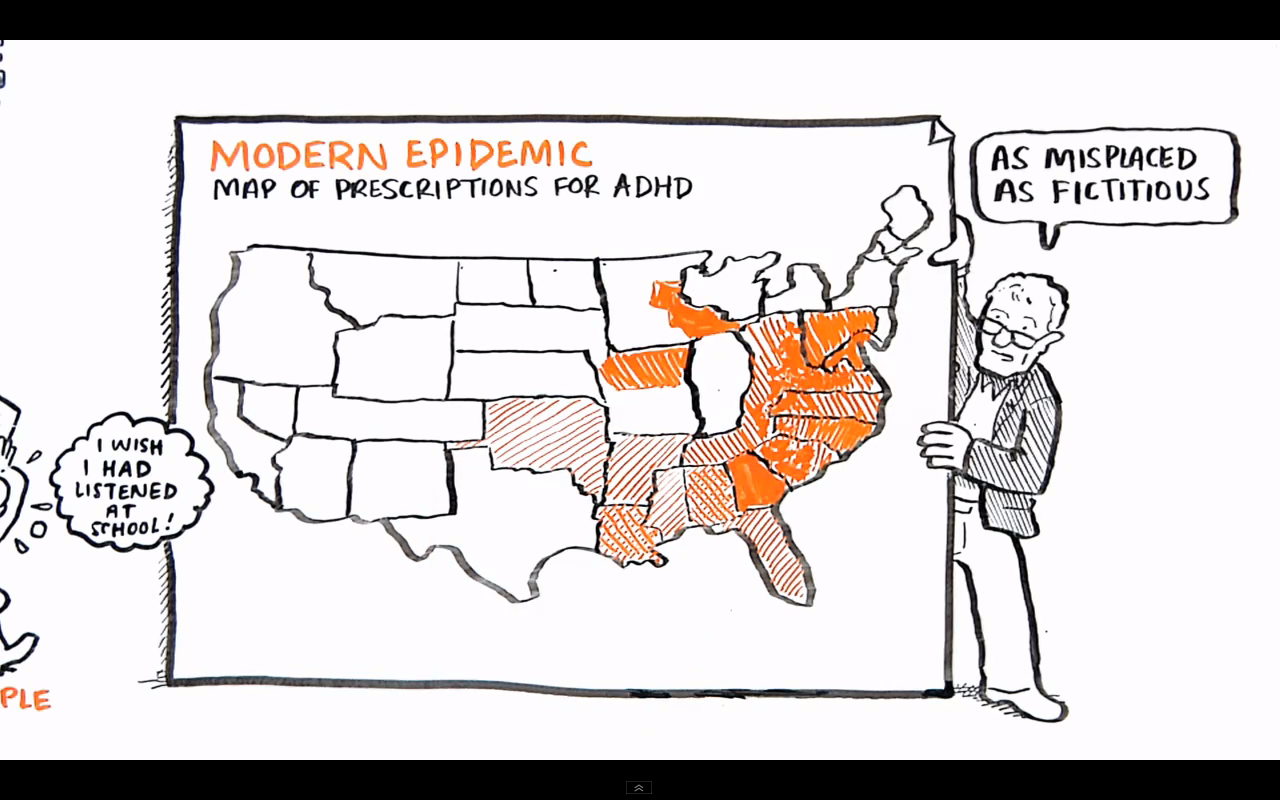
\includegraphics[trim=1.9cm 1.5cm 0cm 1.5cm, clip=true, width=\linewidth]{../resources/illustrations/ADHD}
\label{adhd_map}
%% @todo need caption
\end{figure}
Aussi, ne devrions-nous pas nous demander dans quelle mesure est-il
possible qu'une épidémie de troubles de l'attention touche la nouvelle
génération~? Dans la mesure ou ce trouble n'est lié à aucun virus ou à
aucune bactérie, ne devrions-nous pas mettre en cause le surplus
d'informations dont sont abreuvés nos enfants~? En effet, la nouvelle
génération est née à l'heure où internet et les \gls{ticLabel} sont
omniprésents. Peut-on seulement envisager la possibilité que ce
surplus d'informations empêche les enfants de se focaliser sur des
données jugées inintéressantes tel que les cours magistraux donnés de manière formelle par exemple~?

Ces pistes nous poussent tout naturellement à reconsidérer la manière d'enseigner tout autant que les contenus. Comment intégrer activement les jeunes dans leur éducation, que leur enseigner pour qu'ils évitent les écueils des \gls{ticLabel} ?
Nous allons tout d'abord examiner quelques initiatives existantes allant dans ce sens.

